\documentclass[12pt]{article}
\usepackage{amsfonts, amsmath, amsthm, amssymb}
\usepackage[left=1cm,right=1cm,top=1cm,bottom=2cm]{geometry}
\usepackage{paralist}
\usepackage[russian]{babel}
\usepackage[utf8]{inputenc}
\usepackage{graphicx}

\newcounter{zadacha}
\newcommand{\z}{\par  \smallskip \noindent \refstepcounter{zadacha}%
\textbf{Задача №\arabic{zadacha}.} }

\def\sol{\par \bigskip \noindent \textbf{Решение. }}
\def\solI{\noindent \textbf{Первое решение. }}
\def\solII{\par \noindent \textbf{Второе решение. }}
\def\solIII{\par \noindent \textbf{Третье решение. }}
\def\lemmaI{\noindent \textbf{Лемма. }}
\def\lemma#1{\noindent \textbf{Лемма {#1}. }}
\def\proof{\par \noindent \textbf{Доказательство. }}

\DeclareRobustCommand{\divby}{%
  \mathrel{\text{\vbox{\baselineskip.65ex\lineskiplimit0pt\hbox{.}\hbox{.}\hbox{.}}}}%
}

\begin{document}

\centerline{\sc \textbf{XIX Математическая олимпиада «Шёлковый путь»}}

\centerline{\sc \textbf{Март 2020 года}}

\bigskip
\hrule
\bigskip

\textsl{\textbf{Внимание!} 
Так как XIX Математическая олимпиада «Шёлковый путь» проводится в Казахстане раньше, чем в других странах, мы вас убедительно просим \textbf{не разглашать} эти задачи и не обсуждать их (особенно по Интернету) до 25 мая 2020 года.}

\bigskip

\centerline{\sc \textbf{Решения задач и схемы оценивания}}

\bigskip

\z Дана строго возрастающая бесконечная последовательность натуральных чисел $a_1,$ $a_2,$ $a_3,$ $\ldots$. Известно, что $a_n \leq n + 2020$ и число $n^3 a_n - 1$ делится на $a_{n+1}$ при всех натуральных $n$. Докажите, что $a_n = n$ при всех натуральных $n$. % (\textit{Сатылханов Канат})

\bigskip

\solI Индукцией по $n$ легко показать, что $a_n \geq n$ для любого $n$. Пусть существует такое натуральное $k$, что $a_k > k$. Выберем такое натуральное $m$, что $m \divby 2021!$ и $m > k$. Тогда при всех $i=2, 3, \ldots, 2021$, НОД$(m, m+i) > 1$. Из условия задачи следует, что НОД$(m, a_{m+1})=1$. Так как последовательность $\{a_n\}$ возрастающая и $a_k > k$, то $a_{m+1} > m+1$. Значит, $m + 2 \leq a_{m+1} \leq m + 2021$, но тогда НОД$(m, a_{m+1}) > 1$ --- противоречие.

\bigskip

\textbf{Схема оценивания.}
\begin{compactitem}
\item Рассмотрение натурального числа, делящегося на каждое из чисел $2, 3, \ldots, 2021$ --- 2 балла
\item Доказательство того, что для любого натурального $k$ существует такое натуральное $m > k$, что $a_m = m$ --- 6 баллов
\item Эти пункты не суммируются
\end{compactitem}

\bigskip

\solII Пусть $b_n = a_n - n$ для всех $n$. Индукцией по $n$ легко показать, что $b_n \geq 0$ для любого $n$. Если $b_k > b_{k+1}$ для какого-то $k$, то 
\[a_k - k > a_{k+1} - k - 1 \implies a_k + 1 > a_{k+1} \implies a_k \geq a_{k+1}\]
--- противоречие. Следовательно, последовательность $\{b_n\}$ неубывает. С другой стороны, она ограничена сверху: $b_n = a_n - n \leq 2020$. Следовательно, существует такое неотрицательное целое $k$ и натуральное $t$, что $b_n = k$ для всех $n \geq t$. Значит, для всех $n \geq t$
\[a_{n+1} \ | \ n^3 a_n - 1 \implies n + k + 1 \ | \ n^3 (n + k) - 1 \implies\]
\[\implies n + k + 1 \ | \ n^3 (n + k) - 1 - (n + k + 1)(n^3 - n^2 + n(k+1) - (k+1)^2) = (k + 1)^3 - 1 \implies\]
\[\implies n + k + 1 \ | \ (k + 1)^3 - 1.\]
Но это возможно только если $k = 0$. Следовательно, $b_n = 0$ для всех достаточно больших $n$, а значит и для всех $n$, т. е. $a_n = n$ для всех $n$.

\bigskip

\textbf{Схема оценивания.}
\begin{compactitem}
\item (1) Доказательство того, что $b_k \leq b_{k+1}$ для любого $k$ --- 1 балл
\item (2) Доказательство того, что $\{b_n\}$ постоянна, начиная с какого-то члена --- 3 балла
\item (3) Доказательство того, что $b_n = 0$, начиная с какого-то члена --- 3 балла
\item Пункты (1) и (2) не суммируются
\end{compactitem}

\bigskip

\z Треугольник $ABC$ вписан в окружность $\omega$. На сторонах $AB, BC, CA$ отмечены точки $K, L, M$, соответственно, причем $CM \cdot CL = AM \cdot BL$. Луч $LK$ пересекает прямую $AC$ в точке $P$.  Общая хорда окружности $\omega$ и описанной окружности треугольника $KMP$ пересекает отрезок $AM$ в точке $S$. Докажите, что $SK \parallel BC$. % \textit{(Кунгожин Медеубек)}

\bigskip

\solI 

\bigskip

{
\centerline {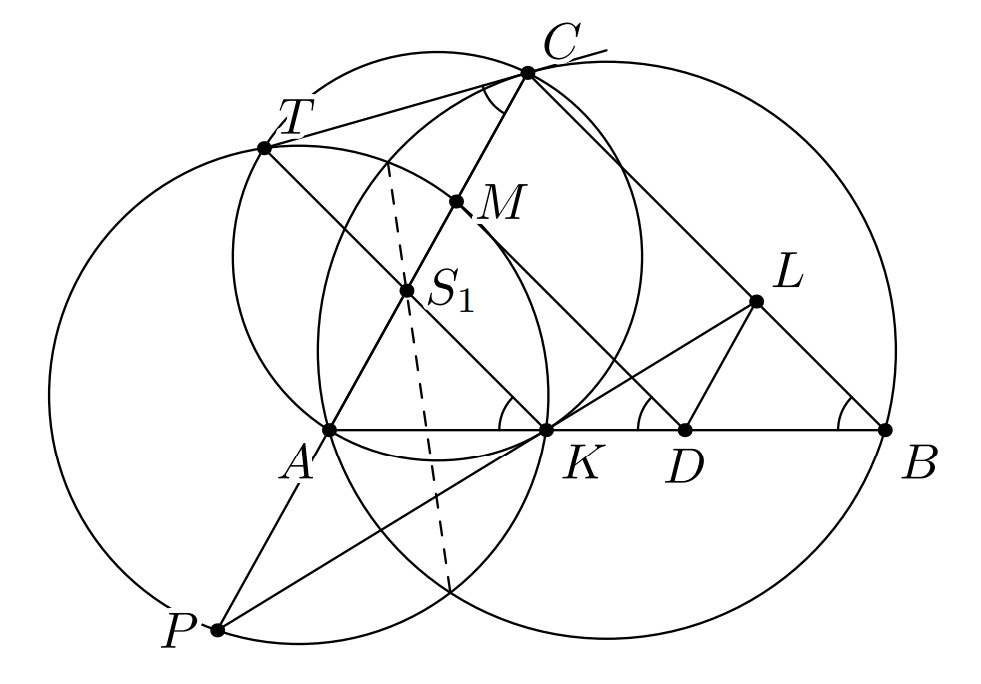
\includegraphics[scale=0.5]{img_1.jpg}}
}

\bigskip

\noindent Пусть $AC \leq BC$. Отметим на стороне $AB$ точку $D$ такую, что $DM \parallel BC$. Тогда 
\[\frac{DB}{DA} = \frac{CM}{AM} = \frac{BL}{CL},\]
то есть $DL \parallel AC$. На касательной прямой к $\omega$ в точке $C$ отметим точку $T$ такую, что $KT \parallel BC$. Тогда $\angle TKA = \angle CBA = \angle TCA$. Следовательно, четырехугольник $AKCT$ --- вписанный. Пусть отрезки $KT$ и $AC$ пересекаются в точке $S_1$. Тогда 
\[\frac{S_1P}{S_1C} = \frac{KP}{KL} = \frac{KA}{KD} = \frac{S_1A}{S_1M} \implies S_1P \cdot S_1M = S_1C \cdot S_1A = S_1K \cdot S_1T.\]
Значит, четырехугольник $TMKP$ вписан в окружность, описанную около треугольника $KMP$. Известно, что общие хорды каждой пары трёх окружностей, центры которых не лежат на одной прямой, пересекаются в одной точке. Это значит, что общая хорда окружности $\omega$ и описанной окружности треугольника $KMP$ проходит через точку $S_1$. Следовательно, точки $S_1$ и $S$ совпадают, и параллельность $S_1K \parallel BC$ верна из построения точки $T$. 

\bigskip

\textbf{Схема оценивания.}
\begin{compactitem}
\item Доказательство того, что $DL \parallel AC$ --- 0 баллов
\item Рассмотрение точки $T$ --- 1 балл
\item Доказательство того, что точки $P, K, M, T$ лежат на одной окружности --- 4 балла
\end{compactitem}

\bigskip

\solII Введем обозначения:
\[b = AC, \ m = AM, \ s = AS, \ p = AP.\]
Так как $S$ лежит на радикальной оси описанных окружностей треугольников $ABC$ и $PKM$, то 
\[SM \cdot SP = SA \cdot SC \implies (m - s)(s + p) = s(b - s) \implies s = \frac{pm}{b + p - m}.\]
Тогда 
\[\frac{AS}{SC} = \frac{s}{b - s} = \frac{pm}{(b - m)(b + p)}.\]
По теореме Менелая для треугольника $ABC$ и секущей $PKL$:
\[\frac{AK}{KB} \cdot \frac{BL}{LC} \cdot \frac{CP}{PA} = 1 \implies \frac{AK}{KB} = \frac{CL}{LB} \cdot \frac{AP}{PC} = \frac{AM}{MC} \cdot \frac{AP}{PC} = \frac{m}{b - m} \cdot \frac{p}{b + p} = \frac{AS}{SC} \implies SK \parallel BC,\]
что и требовалось доказать.

\bigskip

\textbf{Схема оценивания.}
\begin{compactitem}
\item Незаконченный счет --- 0 баллов
\end{compactitem}

\bigskip

\z Многочлен $Q(x) = k_n x^n + k_{n-1} x^{n-1} + \ldots + k_1 x + k_0$ с действительными коэффициентами назовём \textit{мощным}, если выполнено равенство $|k_0| = |k_1| + |k_2| + \ldots + |k_{n-1}| + |k_n|$, и \textit{невозрастающим}, если $k_0 \geq k_1 \geq \ldots \geq k_{n-1} \geq k_n$. 

Пусть для многочлена $P(x) = a_d x^d + a_{d-1} x^{d-1} + \ldots + a_1 x + a_0$ с ненулевыми действительными коэффициентами, где $a_d > 0$, многочлен $P(x)(x-1)^t(x+1)^s$ является \textit{мощным} для некоторых неотрицательных целых $s$ и $t$ ($s + t > 0$). Докажите, что хотя бы один из многочленов $P(x)$ и $(-1)^d P(-x)$ является \textit{невозрастающим}. % \textit{(Navid Safaei, Иран)}

\bigskip

\sol Заметим следующий факт: если для действительных чисел $x_1, x_2, \ldots, x_m$ выполняется равенство
\[|x_1| + |x_2| + \ldots + |x_m| = |x_1 + x_2 + \ldots + x_m|,\]
то они одного знака.

Пусть
\[Q(x) = P(x) (x-1)^t (x+1)^s = b_n x^n + b_{n-1} x^{n-1} + \ldots + b_0,\]
где $b_n = a_d > 0$. Из условия имеем равенство 
\[|b_0 |=|b_1| + |b_2| + \ldots + |b_n|.\]

\textbf{Лемма:} Если $t \geq 1$, то $b_1, b_2, \ldots, b_n \geq 0$.

\textbf{Доказательство:} 
\[Q(1) = 0 \implies b_0 + b_1 + \ldots + b_n = 0 \implies\] 
\[\implies |b_1 + b_2 + \ldots + b_n| = |b_0| = |b_1| + |b_2| + \ldots + |b_n|,\]
а значит, числа $b_1, b_2, \ldots, b_n$ одного знака. Так как $b_n > 0$, то $b_1, b_2, \ldots, b_{n-1} \geq 0$. Лемма доказана.

Предположим, что $t \geq 2$. По лемме,
\[b_1, b_2, \ldots, b_{n-1} \geq 0 \implies b_1 + 2b_2 + \ldots + nb_n > 0.\] 
С другой стороны, пусть $R(x) = \dfrac{Q(x)}{(x - 1)^2}$. Тогда
\[Q'(x) = 2(x - 1) R(x) + (x - 1)^2 R'(x) \implies Q'(1) = 0 \implies b_1 + 2b_2 + \ldots + nb_n = 0\]
--- противоречие. Следовательно, $t \leq 1$.

Аналогично можно показать, что $s \leq 1$. Теперь рассмотрим три случая.

\textbf{I)} $t = 1, s = 1$. 
\[Q(x) = P(x) (x^2 - 1) \implies Q(1) = Q(-1) = 0 \implies \]
\[\implies b_0 + b_1 + \ldots + b_n = b_0 - b_1 + b_2 + \ldots + {(-1)^n} b_n = 0 \implies\]
\[\implies b_1 + b_3 + b_5 + \ldots = 0.\]
По лемме,
\[b_1, b_2, \ldots, b_n \geq 0 \implies b_1 = b_3 = b_5 = \ldots = 0,\]
--- противоречие, так как $b_1 = -a_1$ и по условию $a_1 \ne 0$. 

\textbf{II)} $t = 1, s = 0$.
\[Q(x) = P(x)(x-1) = -a_0 + (a_0 - a_1 ) x + \ldots + (a_{d-1} - a_d) x^d + a_d x^{d+1}.\]
По лемме,
\[a_0 - a_1 = b_1 \geq 0, \ldots, a_{d-1} - a_d = b_d \geq 0 \implies a_0 \geq a_1 \geq \ldots \geq a_d.\]
Следовательно, $P(x)$ --- невозрастающий.

\textbf{III)} $t = 0, s = 1$.
\[Q(-1) = 0 \implies b_0 - b_1 + \ldots + (-1)^n b_n = 0 \implies\]
\[\implies |b_1 - b_2 + \ldots + (-1)^n b_n| = |b_0| = |b_1| + |-b_2| + \ldots + |(-1)^n b_n|.\]
Значит, числа $b_1, -b_2, \ldots, (-1)^n b_n$ одного знака, а так как $b_n > 0$, то $(-1)^{n-i} b_i \geq 0$ для каждого $1 \leq i \leq n$. 
\[Q(x) = P(x)(x+1) = a_0 + (a_0 + a_1) x + \ldots + (a_{d-1} + a_d) x^d + a_d x^{d+1} \implies\]
\[\implies (-1)^{d+1-i} (a_{i-1} + a_i) \geq 0 \ (\text{для всех } 1 \leq i \leq d) \implies\]
\[\implies a_d \leq -a_{d-1} \leq a_{d-2} \leq \ldots \leq (-1)^d a_0.\]
Получается, что многочлен $(-1)^d P(-x) = a_d x^d - a_{d-1} x^{d-1} + \ldots + (-1)^d a_0$ --- невозрастающий.

\bigskip

\textbf{Схема оценивания.}
\begin{compactitem}
\item (1) Доказательство \textbf{леммы} --- 2 балла
\item (2) Доказательство того, что $t \leq 1$ и $s \leq 1$ --- 4 балла
\item (3) Доказательство того, что $t \leq 1$ или $s \leq 1$ --- 3 балла
\item (4) Разбор случая $t = s = 1$ --- 1 балл
\item (5) Разбор случая $t = 1, s = 0$ --- 1 балл
\item (6) Разбор случая $t = 0, s = 1$ --- 1 балл
\item Пункт (1) не суммируется с другими
\item Пункты (2) и (3) не суммируются
\end{compactitem}

\bigskip

\z  Докажите, что для любого натурального числа $m$ существует такое натуральное $n$, что любые $n$ различных точек на плоскости можно разбить на $m$ непустых множеств, \textit{выпуклые оболочки} которых будут иметь общую точку.

\textit{Выпуклой оболочкой} конечного множества $X$ точек на плоскости называется множество точек, лежащих внутри или на границе хотя бы одного выпуклого многоугольника с вершинами в $X$, включая вырожденные, т. е. отрезок и точка считаются выпуклыми многоугольниками. Никакие три вершины выпуклого многоугольника не лежат на одной прямой. Многоугольник содержит свою границу. % (\textit{Зиманов Алихан})

\bigskip

\solI Напомним \textbf{теорему Хелли}: если в конечном множестве выпуклых множеств точек на плоскости каждые три пересекаются, то и все пересекаются.

Докажем, что $n = 9m$ подходит. Пусть $X$ --- произвольное множество из $9m$ различных точек на плоскости, а $Y$ --- множество подмножеств $X$ размера $6m + 1$. 

Предположим, что существуют такие $A, B, C \in Y$, что их пересечение пусто. Пронумеруем все точки из $X$ числами от 1 до $9m$. Выпишем на листе бумаги сначала все номера точек из множества $A$, затем из множества $B$ и в конце из множества $C$. В итоге, мы выпишем $|A| + |B| + |C| = 18m + 3$ числа. Так как эти три множества не пересекаются, то мы не могли выписать никакое число более, чем два раза. Значит, мы выписали не более $2 \cdot 9m = 18m$ чисел --- противоречие. Следовательно, любые три элемента $Y$ пересекаются.

Так как выпуклая оболочка множества точек полностью содержит это множество, то выпуклые оболочки любых трех элементов $Y$ пересекаются. Следовательно, по теореме Хелли, выпуклые оболочки всех элементов $Y$ имеют какую-то общую точку $O$.

Докажем следующую \textbf{лемму}: если выпуклая оболочка какого-то конечного множества точек $Z$ содержит какую-то точку $P$, то существует $W \subseteq Z$, такое что $|W| \leq 3$ и выпуклая оболочка $W$ содержит $P$. По определению выпуклой оболочки, существует выпуклый многоугольник с множеством вершин $V \subseteq Z$ (возможно, вырожденный), который содержит эту точку $P$. Если $|V| \leq 3$, то $V$ подходит в качестве $W$. Иначе, сделаем произвольную триангуляцию многоугольника с вершинами в $V$. Точка $P$ должна лежать хотя бы в одном треугольнике разбиения. Множество вершин такого треугольника подходит в качестве $W$.

Заведем мешок, в который будем складировать непустые подмножества $X$. Определим следующую операцию, изменяющую $X$ и $Y$: выберем любое $A \in Y$. Так как выпуклая оболочка $A$ содержит $O$, то, по лемме, существует такое $B \subseteq A$, что $|B| \leq 3$ и выпуклая оболочка $B$ содержит $O$. Положим $B$ в мешок (очевидно, $B$ непусто), удалим элементы $B$ из $X$, и удалим из $Y$ множества, содержащие элементы $B$. 

После одной операции мощность $X$ уменьшается не более, чем на три, и $Y$ непусто до тех пор, пока $|X| \geq 6m + 1$. Следовательно, мы можем выполнить операцию хотя бы $m$ раз. Выполним операцию ровно $m$ раз. Оставшиеся в $X$ точки распределим произвольным образом между множествами в мешке. 

Итак, множества в мешке составляют разбиение начального множества точек на $m$ множеств и выпуклая оболочка каждого из них содержит точку $O$, т. е. они пересекаются, что нам и было нужно.

\bigskip

\textbf{Схема оценивания.}
\begin{compactitem}
\item Доказательство того, что выпуклые оболочки всех подмножеств размера $\left[\dfrac{2n}{3}\right] + 1$ имеют общую точку --- 3 балла
\item Доказательство \textbf{леммы} --- 1 балл
\item Использование \textbf{леммы} без доказательства --- минус 1 балл
\item Правильно показано, как разбить точки на множества, но без обоснования правильности --- 2 балла
\end{compactitem}

\bigskip

\solII Индукцией по $m$ докажем, что любые хотя бы $4m^2$ различных точек на плоскости можно разбить на $m$ непустых множеств, выпуклые оболочки которых пересекаются. При $m = 1$ утверждение, очевидно, верно. Пусть оно верно для $m = k - 1$, где $k \geq 2$. Докажем, что оно верно и для $m = k$. Рассмотрим произвольное множество $X$ из хотя бы $4k^2$ различных точек на плоскости. Пусть $Y$ --- подмножество точек $X$, лежащих на границе выпуклой оболочки всех точек из $X$. Если $|Y| < 4k$, то $|X \setminus Y| > 4k^2 - 4k > 4(k-1)^2$. По предположению индукции, $X \setminus Y$ можно разбить на $k - 1$ непустое множество точек, выпуклые оболочки которых пересекаются. Если добавить $Y$ к этому $k - 1$ множеству, то мы получим $k$ множеств, выпуклые оболочки которых пересекаются (так как выпуклая оболочка $Y$ содержит все точки из $X \setminus Y$).

Если же $|Y| \geq 4k$, то рассмотрим два случая. Если все точки из $Y$ лежат на одной прямой, то и все точки из $X$ лежат на одной прямой. Проведем вдоль этой прямой ось координат и обозначим точки из $X$ через $A_1, A_2, \ldots, A_{|X|}$ по возрастанию координат. Так как $4k^2 > 2k$, то нам подходит разбиение: 
\[X = \{A_1, A_{|X|}\} \cup \{A_2, A_{|X|-1}\} \cup \ldots \cup \{A_{k-1}, A_{|X|-k+2}\} \cup \{A_k, A_{k+1}, \ldots, A_{|X|-k+1}\}.\]

Иначе, точки $Y$ лежат на границе какого-то невырожденного выпуклого многоугольника. Обозначим точки из $Y$ в порядке обхода по часовой стрелке границы этого многоугольника через 
\[A_1, A_2, \ldots, A_k, B_k, B_{k-1}, \ldots, B_1, C_1, C_2, \ldots, C_k, D_k, D_{k-1}, \ldots, D_1, E_1, E_2, \ldots, E_{|Y| - 4k}.\]
Пусть 
\[Z = \{A_k, B_k, C_k, D_k, E_1, \ldots, E_{|Y| - 4k}\} \cup (X \setminus Y).\]
Докажем, что нам подходит следующее разбиение:
\[X = \left(\bigcup_{i=1}^{k-1} \{A_i, B_i, C_i, D_i\}\right) \cup Z.\]
Для этого достаточно доказать \textbf{ключевое утверждение}: выпуклые оболочки множеств
\[\{A_1, B_1, C_1, D_1\}, \{A_2, B_2, C_2, D_2\}, \ldots, \{A_k, B_k, C_k, D_k\}.\]
пересекаются. Через $f(M)$ будем обозначать выпуклую оболочку множества точек $M$. Пусть
\[T \in A_1B_1 \cap A_kD_k,\]
\[H_i = f(\{A_1, A_2, \ldots, A_i, B_i, B_{i-1}, \ldots, B_1, C_1, C_2, \ldots, C_i, D_i, D_{i-1}, \ldots, D_1\})\]
и
\[V_i = f(\{A_i, A_{i+1}, \ldots, A_k, B_k, B_{k-1}, \ldots, B_i, C_i, C_{i+1}, \ldots, C_k, D_k, D_{k-1}, \ldots, D_i\}).\]
Тогда для любого $1 \leq i \leq k$ верно
\[T \in A_1B_1 \subseteq H_i \ \text{и} \ T \in A_kD_k \subseteq V_i.\]
Следовательно,
\[T \in \bigcap_{i=1}^{k} (H_i \cap V_i) = \bigcap_{i=1}^{k} f(\{A_i, B_i, C_i, D_i\}),\]
что и требовалось доказать.

\bigskip

\textbf{Схема оценивания.}
\begin{compactitem}
\item Сведение к тому, что достаточно доказать \textbf{ключевое утверждение} --- 4 балла
\item Доказательство \textbf{ключевого утверждения} --- 3 балла
\end{compactitem}

\bigskip

\end{document}
